% Cluster analysis
\section{Clustering analysis} \label{s:ap:cs}


\subsection{non-PCA} \label{s:ap:non-pca}


\begin{figure}[!h]
    \captionsetup[subfigure]{justification=Centering}
    \centering
    \begin{subfigure}[!t]{0.3\textwidth}
        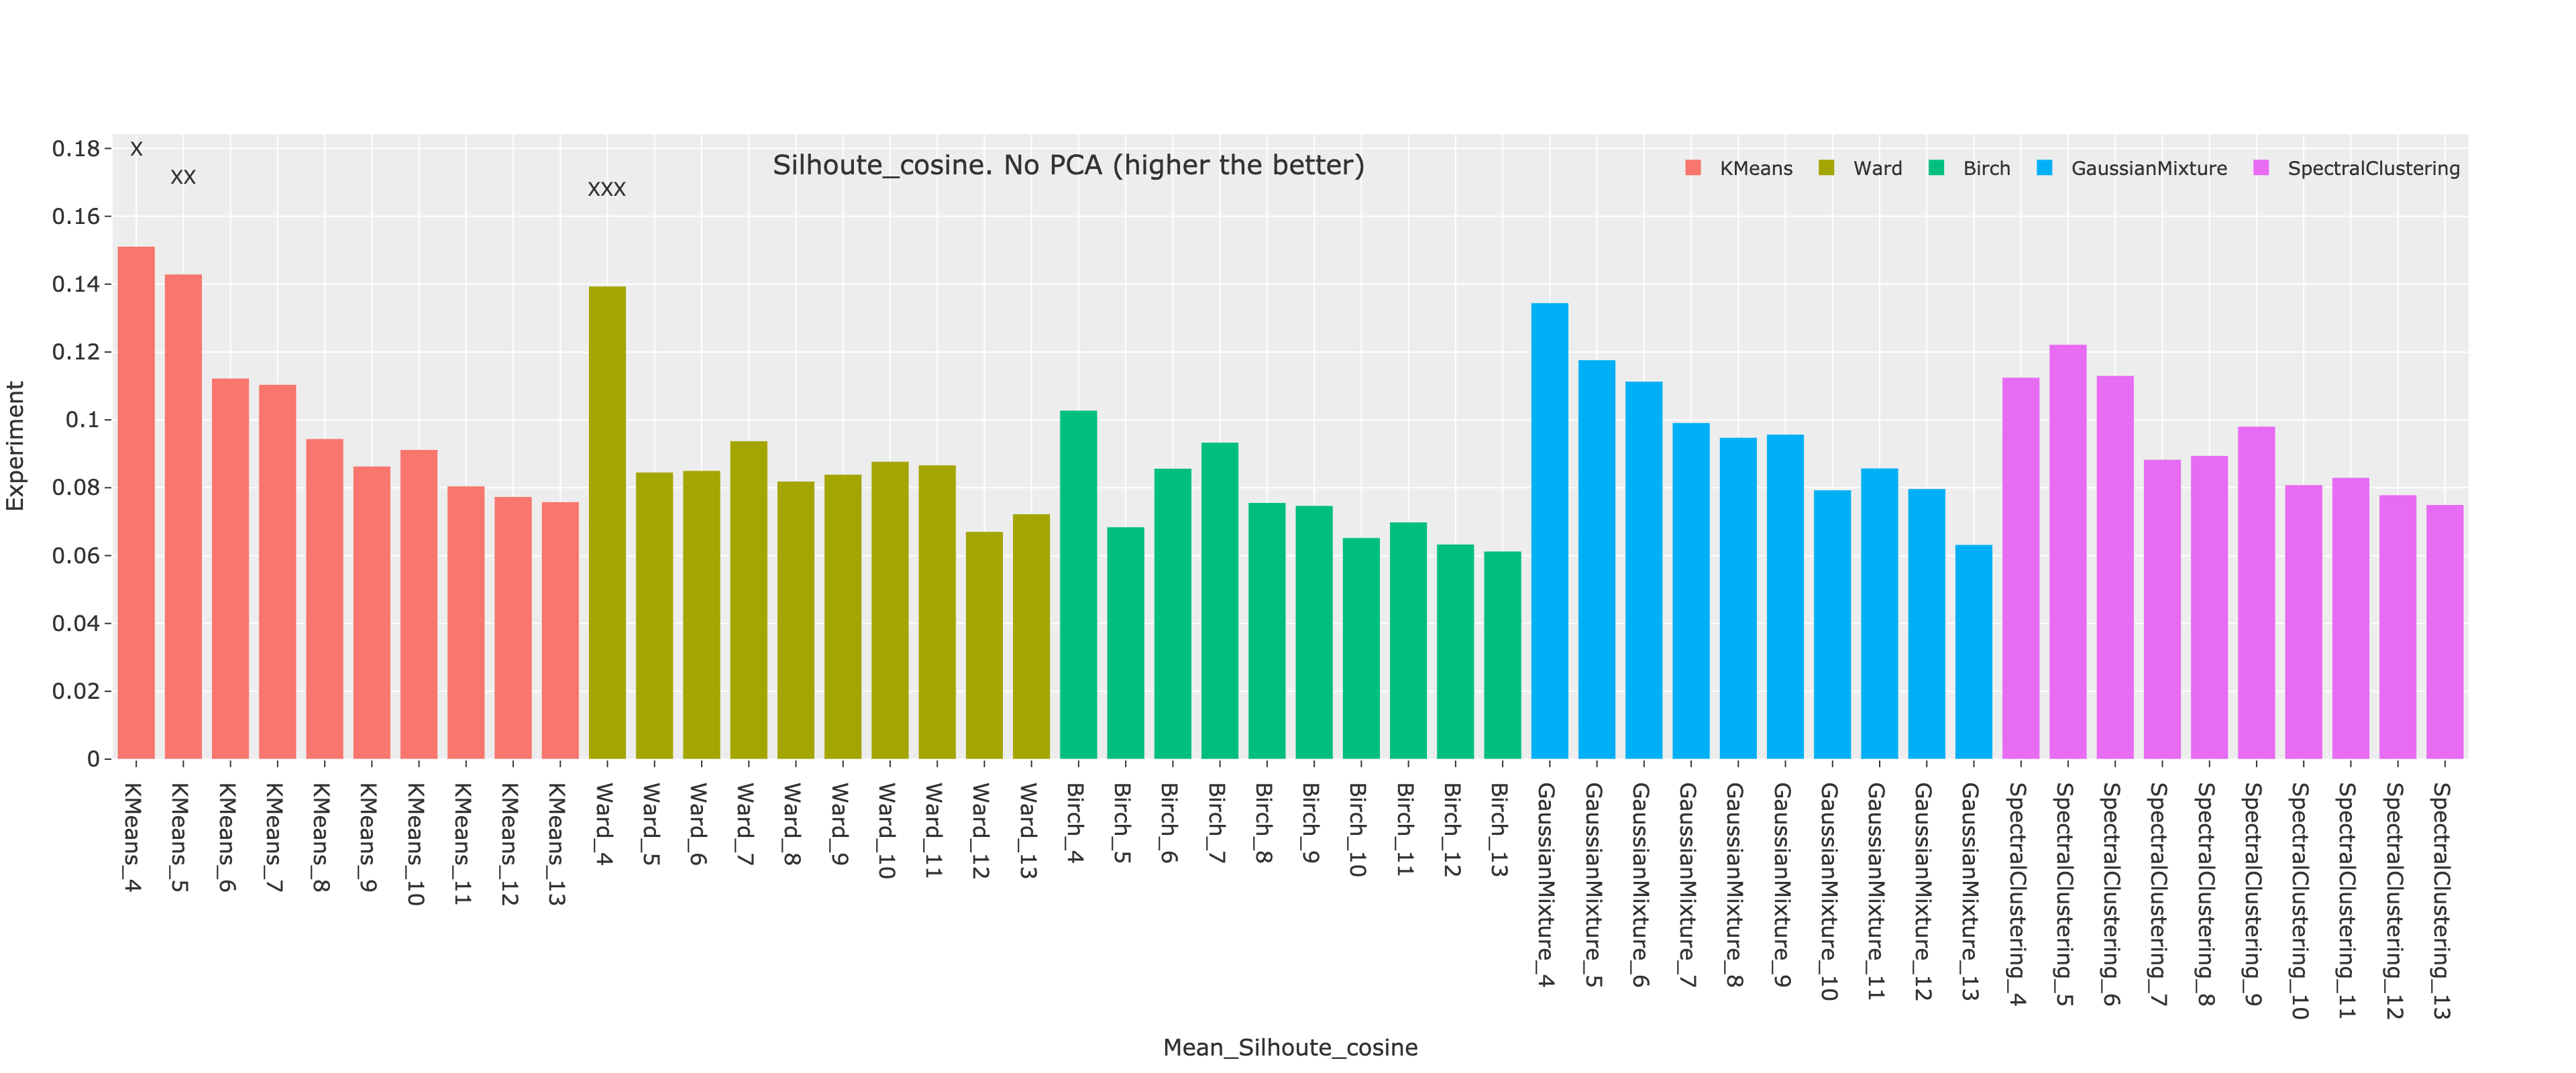
\includegraphics[width=\textwidth]{Sections/ClusteringAnalysis/Resources/cs_top3/nonPCA/non_PCA_top3_Silhoute_cosine.png}
        \caption{Silhouette using cosine distance}
        \label{fig:ap:cosine}
    \end{subfigure}
    \centering
    \begin{subfigure}[!t]{0.3\textwidth}
        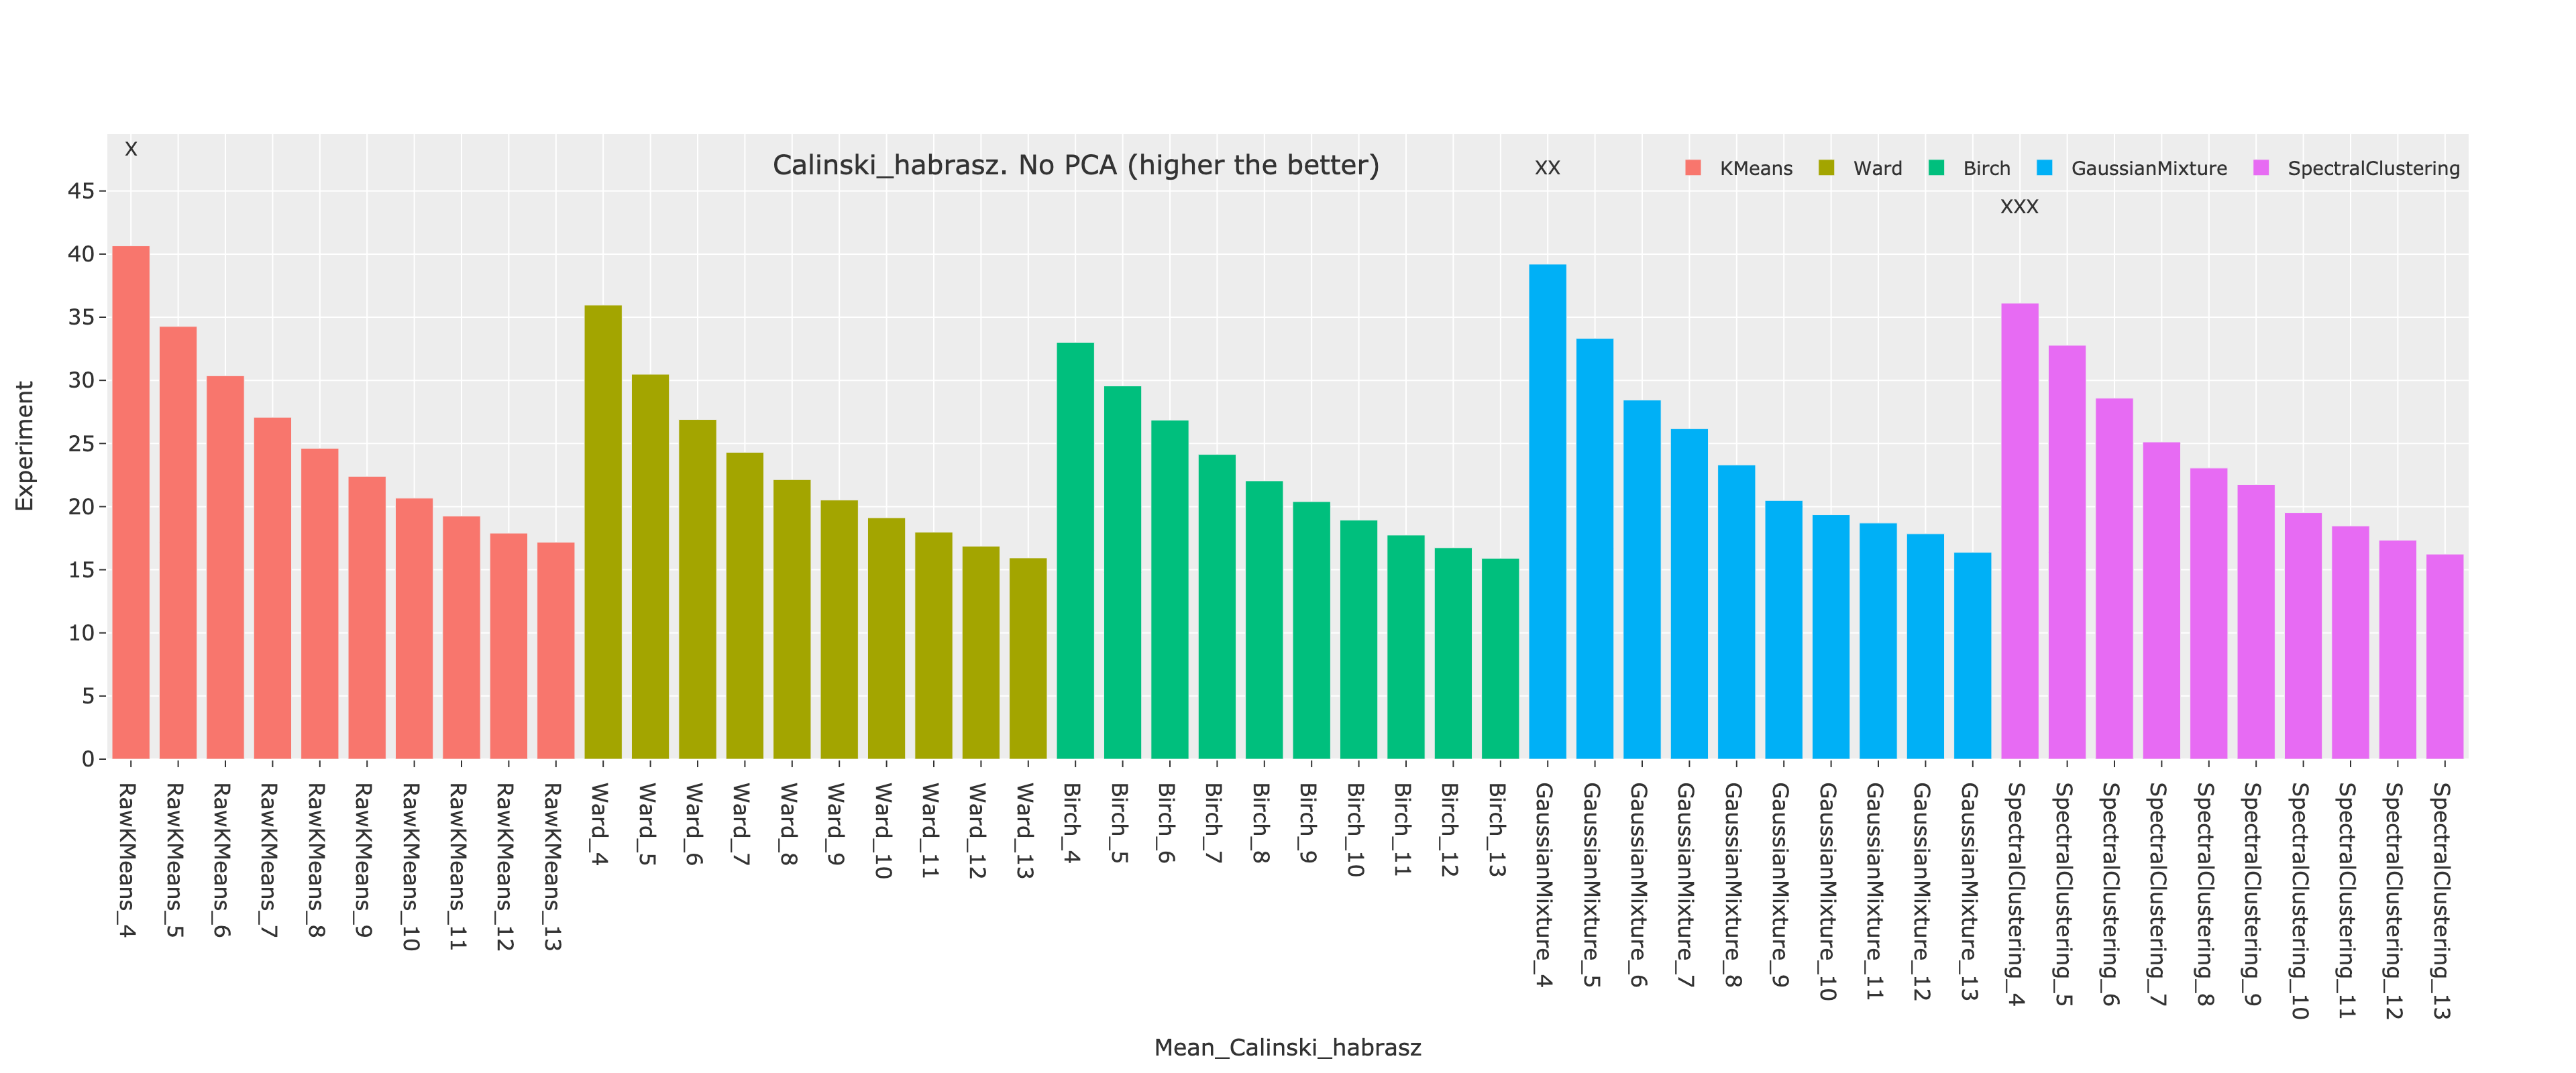
\includegraphics[width=\textwidth]{Sections/ClusteringAnalysis/Resources/cs_top3/nonPCA/non_PCA_top3_Calinski_habrasz.png}
        \caption{Calinski Harabasz}
        \label{fig:ap:cal_hab}
    \end{subfigure}
    \centering
    \begin{subfigure}[!t]{0.3\textwidth}
        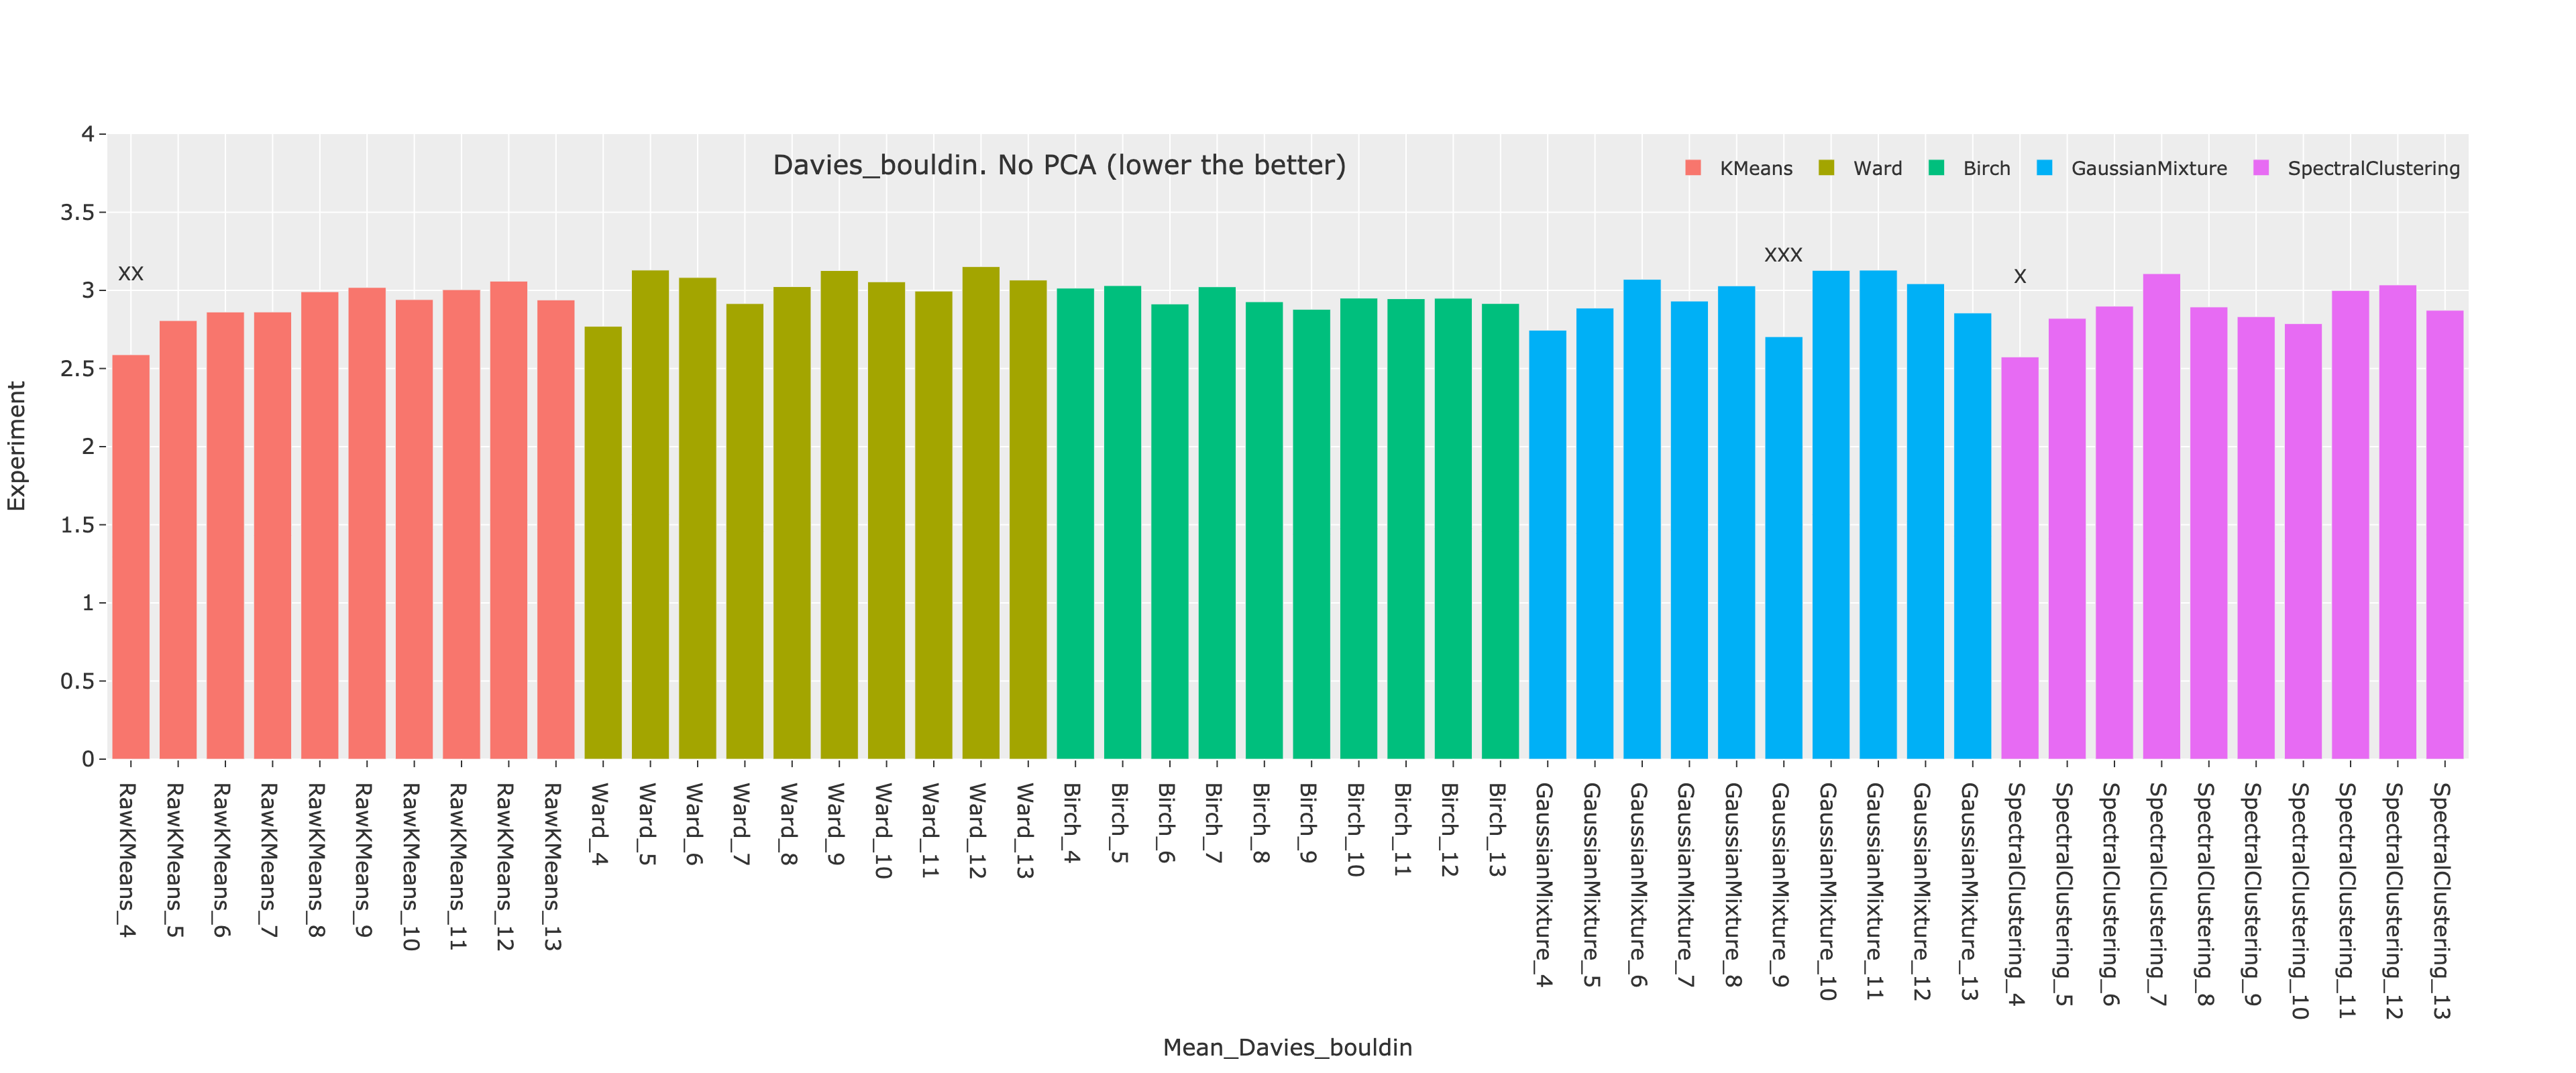
\includegraphics[width=\textwidth]{Sections/ClusteringAnalysis/Resources/cs_top3/nonPCA/non_PCA_top3_Davies_bouldin.png}
        \caption{Davies Bouldin}
        \label{fig:ap:dav_boul}
    \end{subfigure}
    \caption{The means of the three cluster metrics introduced in \cref{s:lit:clustering_metrics}: Silhouette (cosine), Calinski Harabasz and Davies Bouldin. Each of them asses different aspects of clustering and are used to determined the right clustering model for the MIBC cohort from TCGA. The gene expression is processed according to \cref{s:cs:methods} and data was not PCA transformed.}
    \label{fig:ap:non_pca_metrics}
\end{figure}



